\documentclass[11pt]{article}

%####### DON'T CHANGE MARGIN SETTINGS ###########
\newcommand{\keywordfont}{\textsc}
\newcommand{\keyword}[1]{%
  \marginpar{\raggedright\small\keywordfont{#1}}}
\reversemarginpar
\usepackage[a4paper, top=2.5cm, bottom=2.5cm, outer=2cm, inner=3.3cm, marginparwidth=72pt, heightrounded]{geometry}
%#################################
\reversemarginpar
\newcommand{\keywordtwo}[2][0pt]{%
  \marginpar{\vspace*{#1}\raggedright\small\keywordfont{#2}}%
}

\usepackage{amsmath}
\usepackage{amssymb}
\usepackage{amsthm}
\usepackage{hyperref}
\usepackage{graphicx}
\usepackage{microtype}
\usepackage{tikz}
\usepackage{caption}
\usetikzlibrary{trees,positioning,shapes.geometric}

\newtheorem{claim}{Claim}
\newtheorem{conjecture}{Conjecture}




\begin{document}

\Large
\begin{center}
\textbf{MA3K7 Week $6$ Rubric}
\\
Jake O'Bryen (5515129)
\end{center}
\normalsize



\section{Entry}
Immediately from the problem we can see:
There is initially the numbers 1 \keyword{i know}to 2026 within the hat, each of with with an equal probability of being picked. Picking two elements from the hat yields the same result interdependently of the order they are picked, and each time we do this there will be one less number in the hat. This can lead to there being multiple of the same number within the hat. Since you take the difference of two integers, the numbers in the hat will always be non-negative integers between 0 and 2026.

We want to look at the properties \keyword{i want}of the final paper left in the hat, best case i would like to find the distribution of the final number but this may be a tall order. What changes about the hats number composition over time?


\paragraph{Vocabulary.}
\begin{itemize} \keyword{introduce}
    \item call each number inside the hat an 'element' of the hat
    \item call the hat that begins with n numbers, $H^n$, e.g. in the question our hat is $H^{2026}$
    \item call when we pick two numbers and return their difference a 'move', defined by the function $f$, there will only be $N-1$ total moves for $H_k^n(k)$ to return a single element
    \item call the numbers left inside the hat after k moves, $H_k^n$. This is a multiset and non-unique
    \item $\mathbb{H}_k^n(k)$ the multiset of all $H_k^n(k)$
    \item Clearly $f(H_k^n) = H_{k=1}^n$, so $f^p(H_k^n) = H_{k+p}^n$, lets call the final element, $H_{n-1}^n = F $ 
    
\end{itemize}
\section{Attack}
\begin{enumerate} \keywordtwo[7pt]{specialise}
    \item Lets first consider some small cases: $H^3$, $H^4$, $H^5$ $H^6$
    \item lets consider a Monte Carlo simulation for some $n = {10,50,500,2026}$
    \item lets look at a heat map for $(H^n_k)_{k=1}^{k=n-1}$ where n = 2026 to try spot some paterns
    
\end{enumerate}
\noindent
\begin{minipage}[t]{0.4\textwidth}
\vspace{-10pt}

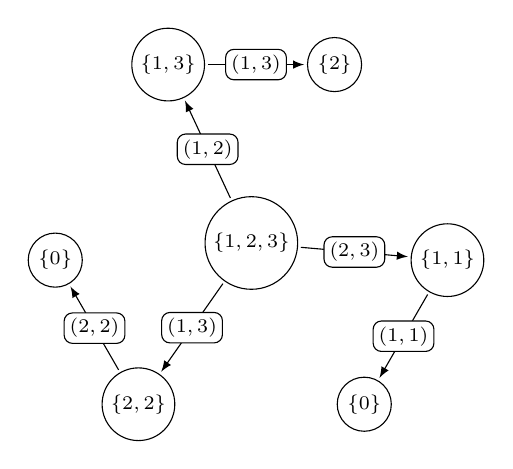
\begin{tikzpicture}[baseline = (current bounding box.north)
  >=latex,
  arr/.style={-latex, shorten <=1pt, shorten >=1pt},
  state/.style={draw, circle, inner sep=2pt, font=\scriptsize, align=center},
  pick/.style={draw, rounded corners=3pt, inner sep=2pt, font=\scriptsize, fill=white, align=center}
]
\def\R{2.5}
\def\delta{25} 

\node[state] (R0) at (0,0) {$\{1,2,3\}$};

\node[state] (S13) at ({90+\delta}:\R) {$\{1,3\}$};
\node[state] (T2)  at ({90-\delta}:\R) {$\{2\}$};

\draw[arr] (R0) -- node[midway,pick] {$(1,2)$} (S13);
\draw[arr] (S13) -- node[midway,pick] {$(1,3)$} (T2);

\node[state] (S22) at ({210+\delta}:\R) {$\{2,2\}$};
\node[state] (T0)  at ({210-\delta}:\R) {$\{0\}$};

\draw[arr] (R0) -- node[midway,pick] {$(1,3)$} (S22);
\draw[arr] (S22) -- node[midway,pick] {$(2,2)$} (T0);

\node[state] (S12) at ({330+\delta}:\R) {$\{1,1\}$};
\node[state] (T1)  at ({330-\delta}:\R) {$\{0\}$};

\draw[arr] (R0) -- node[midway,pick] {$(2,3)$} (S12);
\draw[arr] (S12) -- node[midway,pick] {$(1,1)$} (T1);

\end{tikzpicture}
\captionof{figure}{Distribution tree for $N=3$}

\end{minipage}\hfill\keywordtwo[-5pt]{i find}
\begin{minipage}[t]{0.58\textwidth}

For $N = 3$, we get a fairly simple tree. Since each leaf is equiprobable, we get the following:
\[
\mathbb{P}[F = 0] = 2/3,\quad   \mathbb{P}[F = 2] = 1/3. 
\]
We can use this same idea for $N=4$ with Figure 2 seen below, remembering to account for repeat elements: 
\[
\mathbb{P}[F= 0] = \mathbb{P}[F = 2] = 4/9,\quad \mathbb{P}[F = 4] = 1/9.
\]
Interestingly for $N = 3,4$, we see that $\mathbb{P}[F\text{ is odd}] = 0$, lets see if this pattern continues for larger $N$. Further calculations will rely on python for this as its too complicated to be done by hand
\end{minipage}

\begin{center}

\vspace{-40pt}
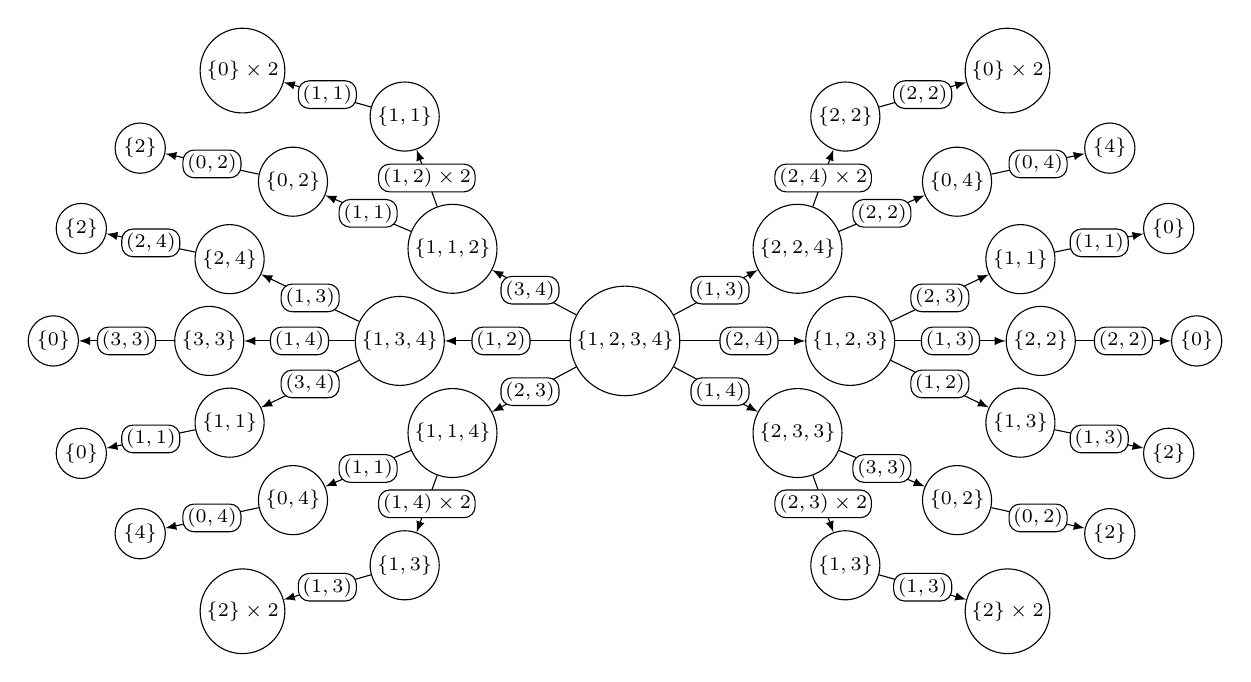
\begin{tikzpicture}[
  xscale=1.1, yscale=0.7,
  >=latex,
  arr/.style={-latex},
  state/.style={draw, circle, inner sep=1.5pt, font=\scriptsize, align=center},
  pick/.style={draw, rounded corners, inner sep=1.5pt, font=\scriptsize, align=center},
]

\def\Rone{2.6}
\def\Rtwo{4.8}
\def\Rthree{6.6}

\def\off{18}

\node[state] (R) at (0,0) {$\{1,2,3,4\}$};

\node[state] (S123) at (0:\Rone)   {$\{1,2,3\}$};  
\node[state] (S134) at (180:\Rone) {$\{1,3,4\}$};  

\node[state] (S224) at (40:\Rone)  {$\{2,2,4\}$};  
\node[state] (S112) at (140:\Rone) {$\{1,1,2\}$};  
\node[state] (S114) at (220:\Rone) {$\{1,1,4\}$};  
\node[state] (S233) at (320:\Rone) {$\{2,3,3\}$};

\draw[arr] (R) -- node[pos=.55,pick,fill=white] {$(2,4)$} (S123);
\draw[arr] (R) -- node[pos=.55,pick,fill=white] {$(1,2)$} (S134);

\draw[arr] (R) -- node[pos=.55,pick,fill=white] {$(1,3)$} (S224);
\draw[arr] (R) -- node[pos=.55,pick,fill=white] {$(3,4)$} (S112);
\draw[arr] (R) -- node[pos=.55,pick,fill=white] {$(2,3)$} (S114);
\draw[arr] (R) -- node[pos=.55,pick,fill=white] {$(1,4)$} (S233);

\node[state] (E13) at ({0-\off}:\Rtwo) {$\{1,3\}$};
\node[state] (E22) at ({0}:\Rtwo)      {$\{2,2\}$};
\node[state] (E11) at ({0+\off}:\Rtwo) {$\{1,1\}$};

\draw[arr] (S123) -- node[midway,pick,fill=white] {$(1,2)$} (E13);
\draw[arr] (S123) -- node[midway,pick,fill=white] {$(1,3)$} (E22);
\draw[arr] (S123) -- node[midway,pick,fill=white] {$(2,3)$} (E11);

\node[state] (TE2)  at ({0-\off}:\Rthree) {$\{2\}$};
\node[state] (TE0a) at ({0}:\Rthree)      {$\{0\}$};
\node[state] (TE0b) at ({0+\off}:\Rthree) {$\{0\}$};

\draw[arr] (E13) -- node[midway,pick,fill=white] {$(1,3)$} (TE2);
\draw[arr] (E22) -- node[midway,pick,fill=white] {$(2,2)$} (TE0a);
\draw[arr] (E11) -- node[midway,pick,fill=white] {$(1,1)$} (TE0b);

\node[state] (A24) at ({180-\off}:\Rtwo) {$\{2,4\}$};
\node[state] (A33) at ({180}:\Rtwo)      {$\{3,3\}$};
\node[state] (A11) at ({180+\off}:\Rtwo) {$\{1,1\}$};

\draw[arr] (S134) -- node[midway,pick,fill=white] {$(1,3)$} (A24);
\draw[arr] (S134) -- node[midway,pick,fill=white] {$(1,4)$} (A33);
\draw[arr] (S134) -- node[midway,pick,fill=white] {$(3,4)$} (A11);

\node[state] (TA2)  at ({180-\off}:\Rthree) {$\{2\}$};
\node[state] (TA0a) at ({180}:\Rthree)      {$\{0\}$};
\node[state] (TA0b) at ({180+\off}:\Rthree) {$\{0\}$};

\draw[arr] (A24) -- node[midway,pick,fill=white] {$(2,4)$} (TA2);
\draw[arr] (A33) -- node[midway,pick,fill=white] {$(3,3)$} (TA0a);
\draw[arr] (A11) -- node[midway,pick,fill=white] {$(1,1)$} (TA0b);

\node[state] (B04) at ({55-\off}:\Rtwo) {$\{0,4\}$};
\node[state] (B22) at ({40+\off}:\Rtwo) {$\{2,2\}$};

\draw[arr] (S224) -- node[midway,pick,fill=white] {$(2,2)$} (B04);
\draw[arr] (S224) -- node[midway,pick,fill=white] {$(2,4) \times2$} (B22);

\node[state] (TB4) at ({50-\off}:\Rthree) {$\{4\}$};
\node[state] (TB0) at ({30+\off}:\Rthree) {$\{0\}\times2$};

\draw[arr] (B04) -- node[midway,pick,fill=white] {$(0,4)$} (TB4);
\draw[arr] (B22) -- node[midway,pick,fill=white] {$(2,2)$} (TB0);

\node[state] (F02) at ({125+\off}:\Rtwo) {$\{0,2\}$};
\node[state] (F11) at ({140-\off}:\Rtwo) {$\{1,1\}$};

\draw[arr] (S112) -- node[midway,pick,fill=white] {$(1,1)$} (F02);
\draw[arr] (S112) -- node[midway,pick,fill=white] {$(1,2)\times2$} (F11);

\node[state] (TF2) at ({130+\off}:\Rthree) {$\{2\}$};
\node[state] (TF0) at ({150-\off}:\Rthree) {$\{0\}\times2$};

\draw[arr] (F02) -- node[midway,pick,fill=white] {$(0,2)$} (TF2);
\draw[arr] (F11) -- node[midway,pick,fill=white] {$(1,1)$} (TF0);

\node[state] (D04) at ({235-\off}:\Rtwo) {$\{0,4\}$};
\node[state] (D13) at ({220+\off}:\Rtwo) {$\{1,3\}$};

\draw[arr] (S114) -- node[midway,pick,fill=white] {$(1,1)$} (D04);
\draw[arr] (S114) -- node[midway,pick,fill=white] {$(1,4)\times2$} (D13);

\node[state] (TD4) at ({230-\off}:\Rthree) {$\{4\}$};
\node[state] (TD2) at ({210+\off}:\Rthree) {$\{2\}\times2$};

\draw[arr] (D04) -- node[midway,pick,fill=white] {$(0,4)$} (TD4);
\draw[arr] (D13) -- node[midway,pick,fill=white] {$(1,3)$} (TD2);

\node[state] (C02) at ({305+\off}:\Rtwo) {$\{0,2\}$};
\node[state] (C13) at ({320-\off}:\Rtwo) {$\{1,3\}$};

\draw[arr] (S233) -- node[midway,pick,fill=white] {$(3,3)$} (C02);
\draw[arr] (S233) -- node[midway,pick,fill=white] {$(2,3) \times 2$} (C13);

\node[state] (TC2a) at ({310+\off}:\Rthree) {$\{2\}$};
\node[state] (TC2b) at ({330-\off}:\Rthree) {$\{2\} \times 2$};

\draw[arr] (C02) -- node[midway,pick,fill=white] {$(0,2)$} (TC2a);
\draw[arr] (C13) -- node[midway,pick,fill=white] {$(1,3)$} (TC2b);


\end{tikzpicture}
\vspace{-25pt}
\captionof{figure}{Distribution tree for $N=4$}
\end{center}
\keywordtwo[32pt]{conjecture}
\keywordtwo[16pt]{stuck}
\noindent
\begin{minipage}[t]{0.52\textwidth}
Reassuringly this gives the same result for $N=4$. For $N=5,6$ we see $\mathbb{P}[F\text{ is even}] = 0$. Maybe we can find a way to determine whether \textbf{F must be even or odd for each N}. 

We can see that the complexity of calculating each case deterministically has increased massively, this is reflected in the runtime of my code. This will be problematic when trying to find larger values of n, especially 2026 even with the aid of python. Lets try a Monte carlo approximation.

\end{minipage}\hfill
\begin{minipage}[t]{0.45\textwidth}
\vspace{0pt}
\centering
\includegraphics[width=\linewidth]{hat_table.png}
\captionof{figure}{Dist. of $F$ for $N = 4,5,6$ (2DP)}
\end{minipage}
\vspace{5pt}

\noindent
Our Monte Carlo simulation seems to show that the probability density is mostly around the smaller numbers, it\keyword{conjecture} also looks as if \textbf{The probability density function is decreasing as k increases}. It also reinforces our idea that F can only ever be even or odd.

\begin{figure}[h]
    \centering
    \includegraphics[width=1\linewidth]{hat1800.png}
    \captionof{figure}{Monte Carlo for $N = 10,50,500,2026$ with 10000 simulations}
    \label{fig:placeholder}
\end{figure}


Looking at the \keyword{idea}number of branches in our examples, each $H^K_i$ produces $|{H^K_i}|\choose2$ non-unique children, formally:
\[
|f(H)| = {|H|\choose2} \quad \text{This could be useful to calculate }  |\mathbb{H}^n_k|\]\keyword{conjecture}
\[
\text{ which may explain \textbf{Why }}\mathbb{P}(F = k) \textbf{ is so hard to calculate} 
\]

\noindent
\begin{minipage}[h]{0.3\textwidth}
\vspace{0pt}
\centering
\includegraphics[width=\linewidth]{heatmap.png}
\end{minipage}\keywordtwo[-25pt]{conjecture}
\begin{minipage}[h]{0.65\textwidth}

I think this provides some solid insight. We can see that larger numbers seem to leave the hat sooner on average This may be because \textbf{Once the largest value leaves the hat it can no longer be re-added}. This will certainly contribute towards larger numbers being less probable. 
We can also see that overall the distribution is lighter further down, but this is obvious because the number of elements in the hat is reduced.

\captionof{figure}{Heat map of how $H^{2026}$ changes over $f$, 5000 trials}

\end{minipage}

\section{Solution}



\begin{claim}For each n, F can only take either positive or negative values

\end{claim}

\begin{proof}
Let $S$ denote the sum of all numbers currently in the bag. Suppose we perform one move,
replacing $a$ and $b$ by $|a-b|$. The new sum is
\[
S' = S-a-b+|a-b|.
\]
Working modulo $2$, note that $|a-b|\equiv a-b\pmod 2$, and since $-b\equiv b\pmod 2$ we have
$a-b\equiv a+b\pmod 2$. Hence
\[
|a-b|\equiv a+b \pmod 2.
\]
Therefore,
\[
S' \equiv S-a-b+(a+b)\equiv S \pmod 2,
\]
so the parity of $S$ is invariant throughout the process.

At the end, a single number $F$ remains, so $S=F$ at termination. Thus
\[
F \equiv S \equiv \sum_{k=1}^n k = \frac{n(n+1)}{2}\pmod 2,
\]
as required. Since
\[
\quad\frac{2026(2026+1)}{2} = 1 \pmod{2},\quad \text{$F$ will always be odd}
\]
\end{proof}

\begin{proof}
Let $H_t$ be the multiset of values in the hat after $t$ merges, and write
\[
M_t:=\max(H_t).
\]
\[
\text{A move replaces } a,b\in H_t \text{ by } c=\lvert a-b\rvert, \text{ so }
\lvert a-b\rvert \le \max\{a,b\}\le M_t.
\]
hence every element of $H_{t+1}$ is $\le M_t$ and therefore $M_{t+1}\le M_t$.

Now suppose the largest value $M_t$ is not present after the merge, i.e.\ $M_t\notin H_{t+1}$.
Then $M_{t+1}<M_t$. By monotonicity of the maximum,
\[
M_s \le M_{t+1} < M_t \qquad \text{for all } s\ge t+1.
\]
Thus no later hat $H_s$ can contain $M_t$, so once the maximum disappears it can never be reintroduced. \qedhere
\end{proof}
    


\begin{claim}For probable values of k, the probability density function is decreasing as k increases
\end{claim}
whilst i am almost certain this is true, i could find no way of proving it. 
\begin{claim}There are $\sim 4\pi\left(\frac{(n-1)^2}{2e^2}\right)^{n-1}$ ways of finding $\mathbb{P}(F = k)$


\end{claim}
Consider a string $H^n$, then $|f(H^n)| = {n\choose2}$ eg there are $\frac{n(n-1)}{2}$ different ways of creating a child string from it. Since we have to apply $f$ n-1 times to find the final value, F. This means there are 
\[
P(n)\;:=\prod^{n-1}_{i=2}{n\choose2} = \prod^{n-1}_{i=2}\frac{n(n-1)}{2} = \frac{(n-1)!(n-2)!}{2^{n-2}}
\] 
different ways of finding our final value F. Lets use Stirling formula with remainder: for every integer $m\ge 1$ there exists $\theta_m\in(0,1)$ such that
\[
m!\;=\;\sqrt{2\pi m}\left(\frac{m}{e}\right)^m
\exp\!\left(\frac{\theta_m}{12m}\right).
\]
Apply this to $m=n-1$ and $m=n-2$:
\[
P(n)
=\frac{1}{2^{n-2}}\sqrt{2\pi (n-1)}\left(\frac{n-1}{e}\right)^{n-1}
\sqrt{2\pi(n-2)}\left(\frac{n-2}{e}\right)^{n-2}
\exp\!\left(\frac{\theta_{n-1}}{12(n-1)}+\frac{\theta_{n-2}}{12(n-2)}\right).
\]
Rearrange:
\[
P(n)
=(2\pi)\,\frac{\sqrt{(n-1)(n-2)}}{2^{n-2}}\,
\frac{(n-1)^{n-1}(n-2)^{n-2}}{e^{2n-3}}\,
\exp\!\left(\frac{\theta_{n-1}}{12(n-1)}+\frac{\theta_{n-2}}{12(n-2)}\right).
\]
Equivalently,
\[
P(n)
=4\pi\left(\frac{(n-1)^2}{2e^2}\right)^{n-1}\,R_n,\quad
R_n
:=e\,
\left(1-\frac{1}{n-1}\right)^{n-{3/2}}
\exp\!\left(\frac{\theta_{n-1}}{12(n-1)}+\frac{\theta_{n-2}}{12(n-2)}\right).
\]
As $n\to\infty$, we have $\widetilde R_n\to 1$, hence
\[
P(n)\sim 4\pi\left(\frac{(n-1)^2}{2e^2}\right)^{n-1}.
\]
A strong dependence on the previous move means we cannot take any shortcuts, making this incredibly difficult to calculate, with this difficulty increasing super exponentially as n increases.




    




\section{Review}
I have given many reasons as \keyword{check}for why this question would be hard to solve, and what makes properties of F so elusive, as other then the trivial properties of F, eg its a non zero integer between 0 and 2026. I didnt manage to show much.

I feel like i was \keyword{reflect}unable to prove much in this assingment, this may be because of its less analytical nature. Unlike the first two assignments, proving what i would call the main idea would be way out of scope for the assignment. This means I could only discuss properties of the question. Python was an excelent aid for such questions though, as the quetsion was very dependant on a lot of menial computation

Throughout \keyword{generalise}the question we considered what would happen for a hat with N starting elements, so we immediately generalised the question. An adaptation we could consider is, instead of picking two elements $(a,b)$ and taking the absolute difference; What if we just considered $a-b$? This would expand the question into allowing F to take negative values and also values greater then the largest original number, N. Since the move is linear, every entry in the hat remains an integer linear combination of the initial $\{1,2,\dots,n\}$ with coefficients in $\{\pm1\}$. so $F_n$ can be represented in the following way

\begin{equation}\label{eq:signed-rep}
X_n=\sum_{k=1}^n k\,\varepsilon_k,\qquad \varepsilon_k\in\{+1,-1\}.
\end{equation}

Each $\varepsilon_k$ is Rademacher: If we swap the subtraction order at every
step (replace each $(a,b)$ by $(b,a)$), then every difference changes sign and therefore
$F_n\mapsto -F_n$. Since ordered choices $(a,b)$ and $(b,a)$ are equally likely, the law of $X_n$
is symmetric:
\[
\mathbb P(F_n=k)=\mathbb P(F_n=-k)\qquad(\forall k\in\mathbb Z),
\]
which forces
\[
\mathbb P(\varepsilon_k=+1)=\mathbb P(\varepsilon_k=-1)=\frac12\qquad(1\le k\le n).
\]
However, the signs are \emph{not independent}: the merge history couples them.
(e.g.\ for $n=2$ one always has $(\varepsilon_1,\varepsilon_2)\in\{(+,-),(-,+)\}$, so
$\mathbb P(\varepsilon_1=\varepsilon_2)=0$).

we can see the sign vector $\varepsilon=(\varepsilon_1,\dots,\varepsilon_n)$ is exchangeable for any permutation $\pi$ of $\{1,\dots,n\}$,
\[
(\varepsilon_1,\dots,\varepsilon_n)\overset{d}{=}(\varepsilon_{\pi(1)},\dots,\varepsilon_{\pi(n)}),
\]
because the dynamics does not use the labels except as names.


\noindent
\begin{minipage}[t]{0.52\textwidth}
 why fig 6 looks Gaussian: Writing
$P=\{k:\varepsilon_k=+1\}$ and $M=|P|$, we have
\[
X_n=\sum_{k\in P}k-\sum_{k\notin P}k \;=\;2\sum_{k\in P}k-\sum_{k=1}^n k
\;=\;2T_M-S,
\]
where $S=\sum_{k=1}^n k$ and $T_M:=\sum_{k\in P}k$. By exchangeability, conditional on $M=m$
the set $P$ is uniform over all $m$-subsets of $\{1,\dots,n\}$, so $T_m$ is the sum of a simple
random sample without replacement from $\{1,\dots,n\}$. Such sample sums satisfy a finite-population
central limit theorem for $m\asymp n$, so $T_m$ (hence $X_n$) is approximately normal after centring
and scaling. This produces the observed bell-shaped distribution, even though the underlying signs
$\varepsilon_k$ are dependent.

\captionof{figure}{Distribution of $F$ for $N = 50$, $1\times 10^6$ Trials}

\end{minipage}\hfill
\begin{minipage}[t]{0.45\textwidth}
\vspace{0pt}
\centering
\includegraphics[width=\linewidth]{extension.png}

\end{minipage}
\vspace{5pt}

\section*{Code}
The code for this assignment can be found on my GitHub page:\\  
\url{https://github.com/siriwarwick/book/tree/main/Chapter4}

In particular, \texttt{mandelbrot.ipynb} was used to plot fig. 1.

\end{document}